\documentclass[tikz,border=5pt]{standalone}
\usepackage{amsmath}
\usepackage{pgfplots}
\pgfplotsset{compat=1.18}

\begin{document}

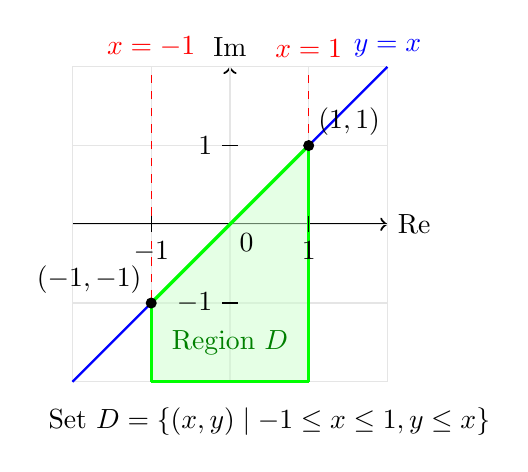
\begin{tikzpicture}
    % Axes
    \draw[->, thick] (-2,0) -- (2,0) node[right] {$\text{Re}$};
    \draw[->, thick] (0,-2) -- (0,2) node[above] {$\text{Im}$};
    
    % Grid
    \draw[gray!20] (-2,-2) grid (2,2);
    
    % Vertical boundaries: x = -1 and x = 1
    \draw[dashed, red] (-1,-2) -- (-1,2) node[above, red] {$x=-1$};
    \draw[dashed, red] (1,-2) -- (1,2) node[above, red] {$x=1$};
    
    % Line y = x
    \draw[blue, thick] (-2,-2) -- (2,2) node[above, blue] {$y=x$};
    
    % Shade the region: y ≤ x AND -1 ≤ x ≤ 1
    \fill[green!20, opacity=0.5] (-1,-2) -- (-1,-1) -- (1,1) -- (1,-2) -- cycle;
    
    % Add boundary lines for the region
    \draw[green, very thick] (-1,-1) -- (1,1);
    \draw[green, very thick] (-1,-1) -- (-1,-2);
    \draw[green, very thick] (1,1) -- (1,-2);
    \draw[green, very thick] (-1,-2) -- (1,-2);
    
    % Dotted line to show the region extends downward
    \draw[green, dotted] (-1,-2) -- (-1,-1.9);
    \draw[green, dotted] (1,-2) -- (1,-1.9);
    
    % Points
    \fill[black] (-1,-1) circle (2pt) node[above left] {$(-1,-1)$};
    \fill[black] (1,1) circle (2pt) node[above right] {$(1,1)$};
    
    % Labels
    \node[green!50!black] at (0,-1.5) {Region $D$};
    \node at (0.5, -2.5) {Set $D = \{(x,y) \mid -1 \leq x \leq 1, y \leq x\}$};
    
    % Origin
    \node at (0,0) [below right] {$0$};
    
    % Scale indicators
    \foreach \x in {-1,1} {
        \draw (\x,0.1) -- (\x,-0.1) node[below] {$\x$};
    }
    \foreach \y in {-1,1} {
        \draw (0.1,\y) -- (-0.1,\y) node[left] {$\y$};
    }
\end{tikzpicture}

\end{document}